% !TEX TS-program = pdflatex
% !TEX encoding = UTF-8 Unicode

% This file is a template using the "beamer" package to create slides for a talk or presentation
% - Giving a talk on some subject.
% - The talk is between 15min and 45min long.
% - Style is ornate.

% MODIFIED by Jonathan Kew, 2008-07-06
% The header comments and encoding in this file were modified for inclusion with TeXworks.
% The content is otherwise unchanged from the original distributed with the beamer package.

\documentclass{beamer}

\mode<presentation>
{
  \usetheme{Malmoe}
  % or ...

  %\setbeamercovered{transparent}
  % or whatever (possibly just delete it)
}


\usepackage[english]{babel}
\usepackage{graphicx}
\usepackage{amssymb}
\usepackage{multicol,multirow,array}
\setbeamertemplate{navigation symbols}{}%remove navigation symbols
\setbeamertemplate{footline}[frame number]


\title[Association Testing with X Chromosome Data] % (optional, use only with long paper titles)
{Association Testing with X Chromosome Data\\
An Application To HCHS/SOL}

%\subtitle
%{Presentation Subtitle} % (optional)

\author[Caitlin McHugh, with Tim Thornton] % (optional, use only with lots of authors)
{Caitlin McHugh, with Tim Thornton}
% - Use the \inst{?} command only if the authors have different
%   affiliation.

\institute[University of Washington] % (optional, but mostly needed)
{
  Department of Biostatistics\\
  University of Washington
}
% - Use the \inst command only if there are several affiliations.
% - Keep it simple, no one is interested in your street address.

\date[Short Occasion] % (optional)
{9 Feb 2015}

% If you have a file called "university-logo-filename.xxx", where xxx
% is a graphic format that can be processed by latex or pdflatex,
% resp., then you can add a logo as follows:

% \pgfdeclareimage[height=0.5cm]{university-logo}{university-logo-filename}
% \logo{\pgfuseimage{university-logo}}

% If you wish to uncover everything in a step-wise fashion, uncomment
% the following command: 

%\beamerdefaultoverlayspecification{<+->}


\begin{document}

\begin{frame}
  \titlepage
\end{frame}

%\begin{frame}{Outline}
 %\tableofcontents
  % You might wish to add the option [pausesections]
%\end{frame}

% Anything you have relevant to the "right" way to do association on the X chromosome in OLGA

\begin{frame}
\begin{columns}
    \begin{column}{0.3\textwidth}
      \centering
      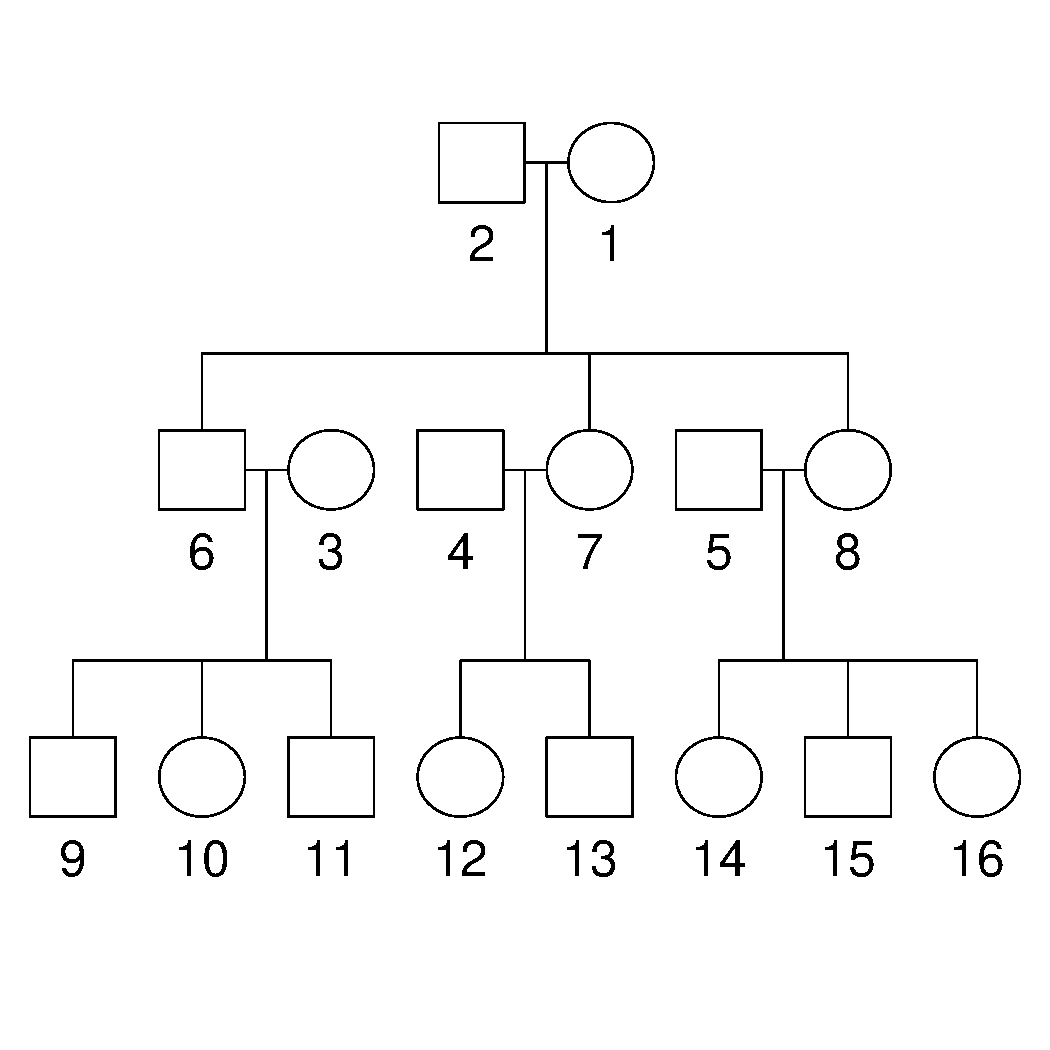
\includegraphics[height=4.5cm]{../pedigree_16individs.pdf}
    \end{column}
    \begin{column}{0.5\textwidth}
      \centering
      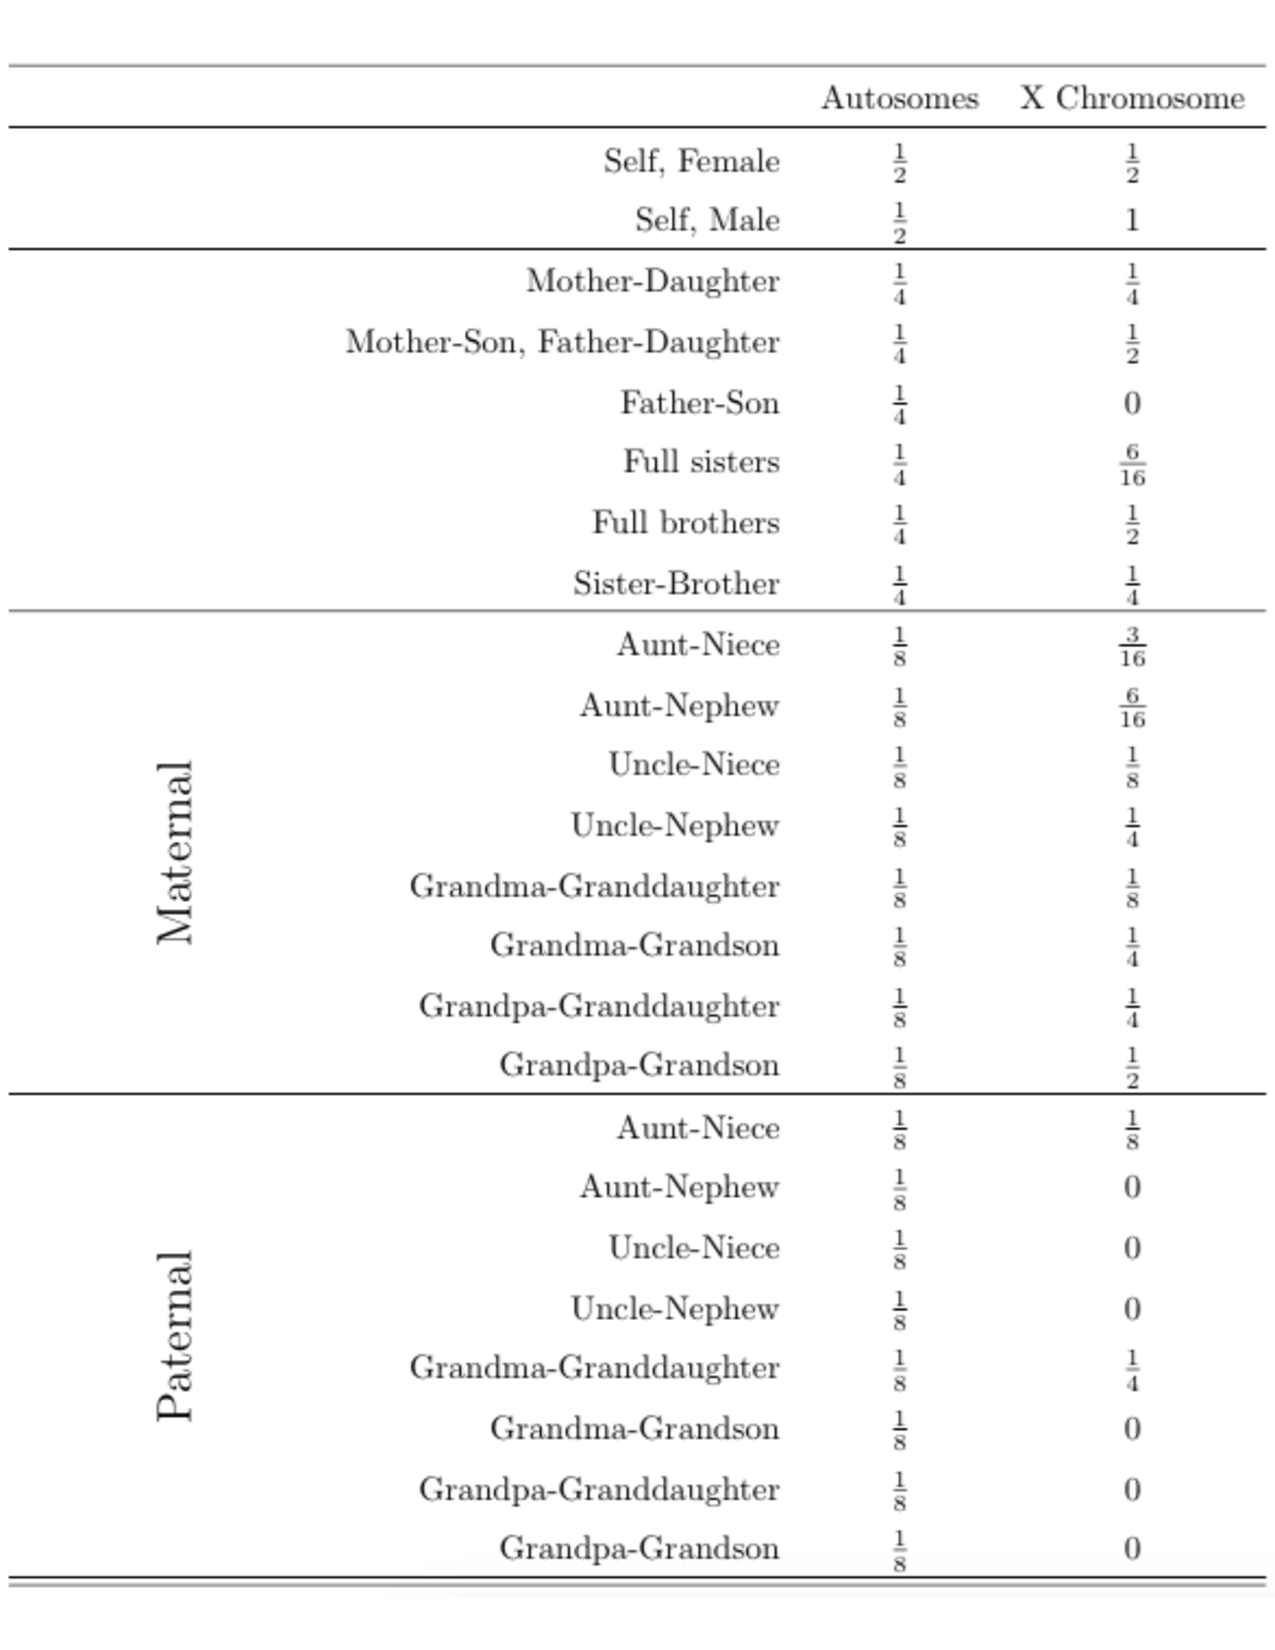
\includegraphics[height=8.3cm]{../olga_presentation_26jan15/xchr_kc_values.pdf}
    \end{column}
 \end{columns}
\end{frame}

\begin{frame}
\begin{itemize}
\item We estimated PCs in the SOL subjects using 3,600 LD-pruned X chromosome SNPs and PC-AiR.
\item The unrelated set \texttt{unrelated.pcair.deg4} of 10,272 samples as defined from the autosomes was set, and only study samples (\texttt{subj.plink \& geno.cntl==0}) excluding \texttt{gengrp6.outliers} were projected for a total of 12,747 samples.
\end{itemize}
\end{frame}

\begin{frame}
\centering
\begin{figure}
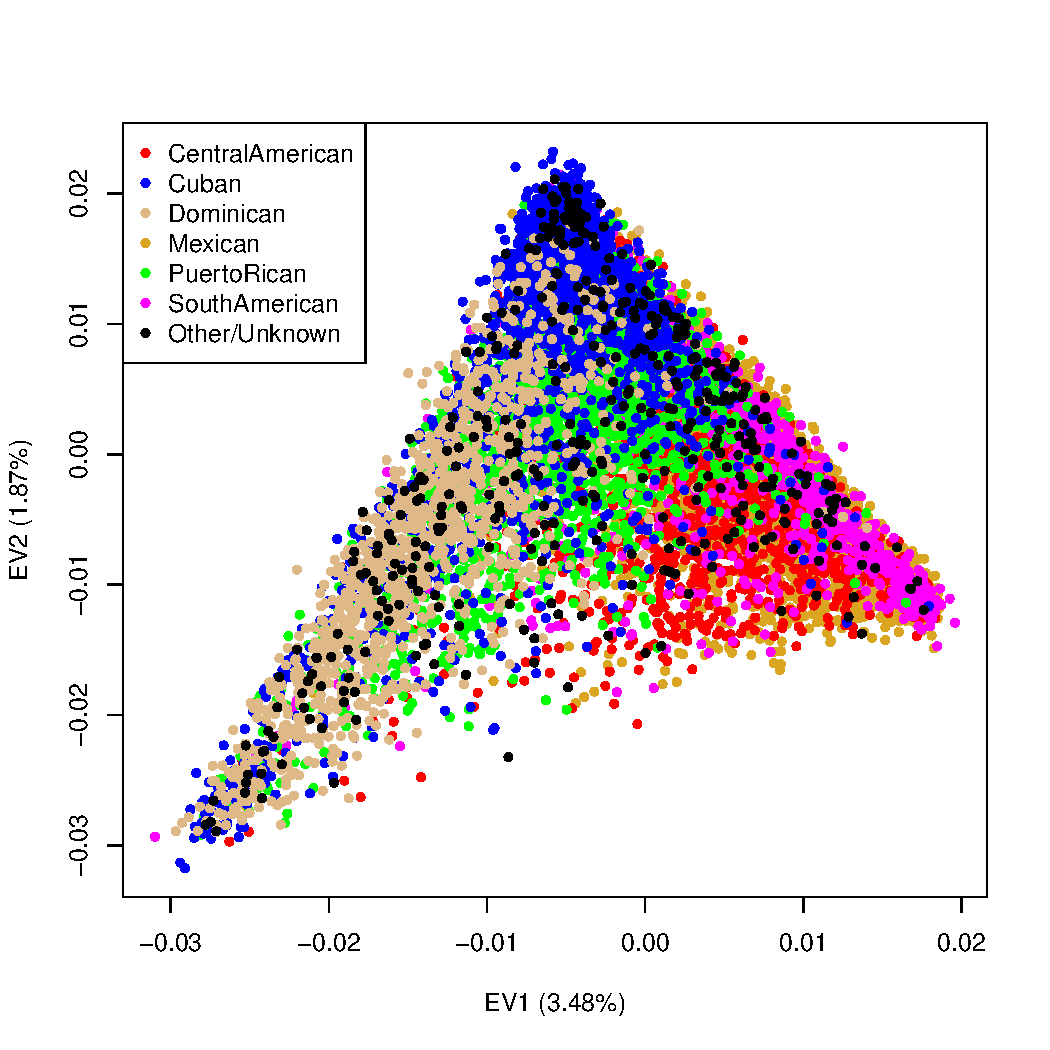
\includegraphics[height=8.5cm]{../pca_x_ev12_col.pdf}
\end{figure}
\end{frame}

\begin{frame}
\centering
\begin{figure}
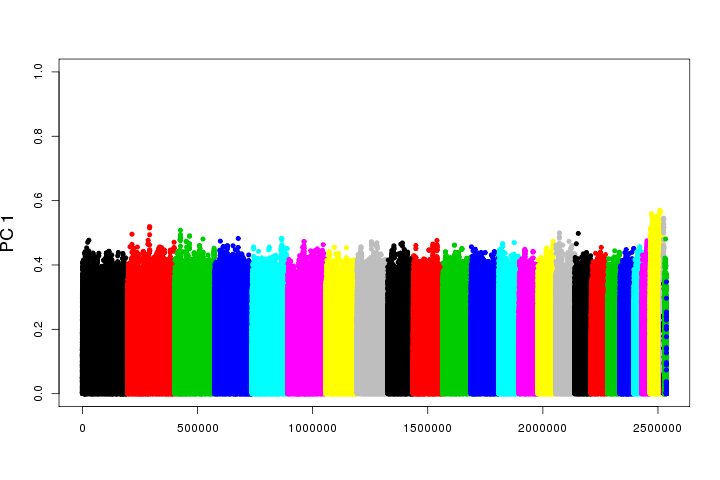
\includegraphics[height=7.5cm]{../pca_x_corrManh_ev1.png}
\end{figure}
\end{frame}

\begin{frame}
\centering
\begin{figure}
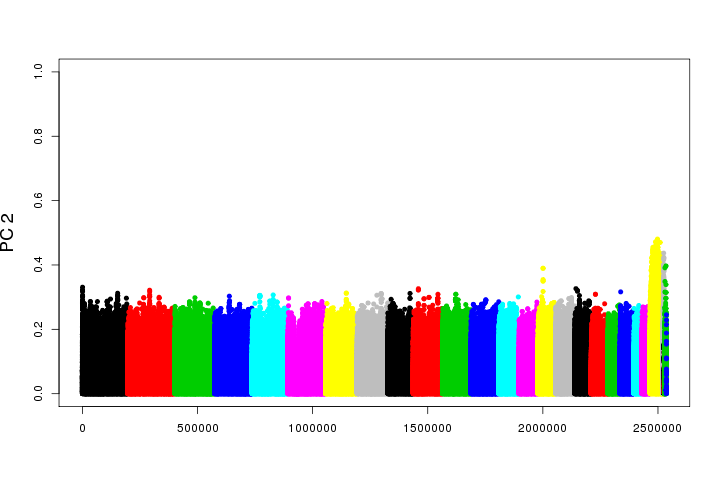
\includegraphics[height=7.5cm]{../pca_x_corrManh_ev2.png}
\end{figure}
\end{frame}

\begin{frame}
\centering
\begin{figure}
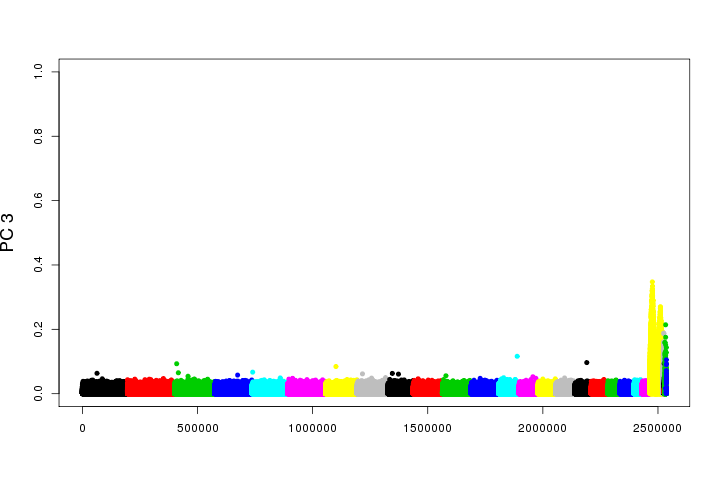
\includegraphics[height=7.5cm]{../pca_x_corrManh_ev3.png}
\end{figure}
\end{frame}

\begin{frame}
\begin{itemize}
\item We compare these results which use only 3,600 X chromosome SNPs to a pruned set of 4,413 chromosome 20 SNPs.
\end{itemize}
\end{frame}


\begin{frame}
\centering
\begin{figure}
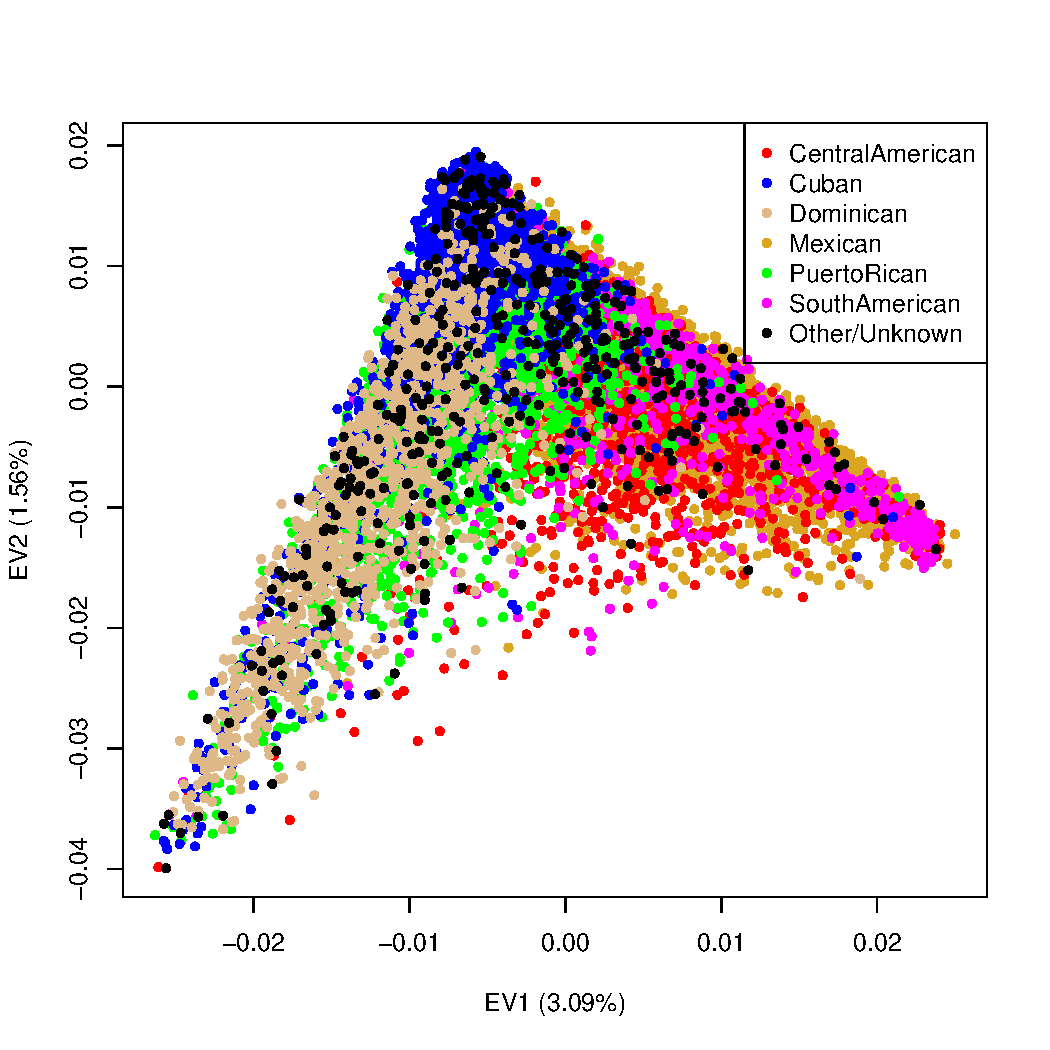
\includegraphics[height=8.5cm]{../pca_chr20_ev12_col.pdf}
\end{figure}
\end{frame}

\begin{frame}
\centering
\begin{figure}
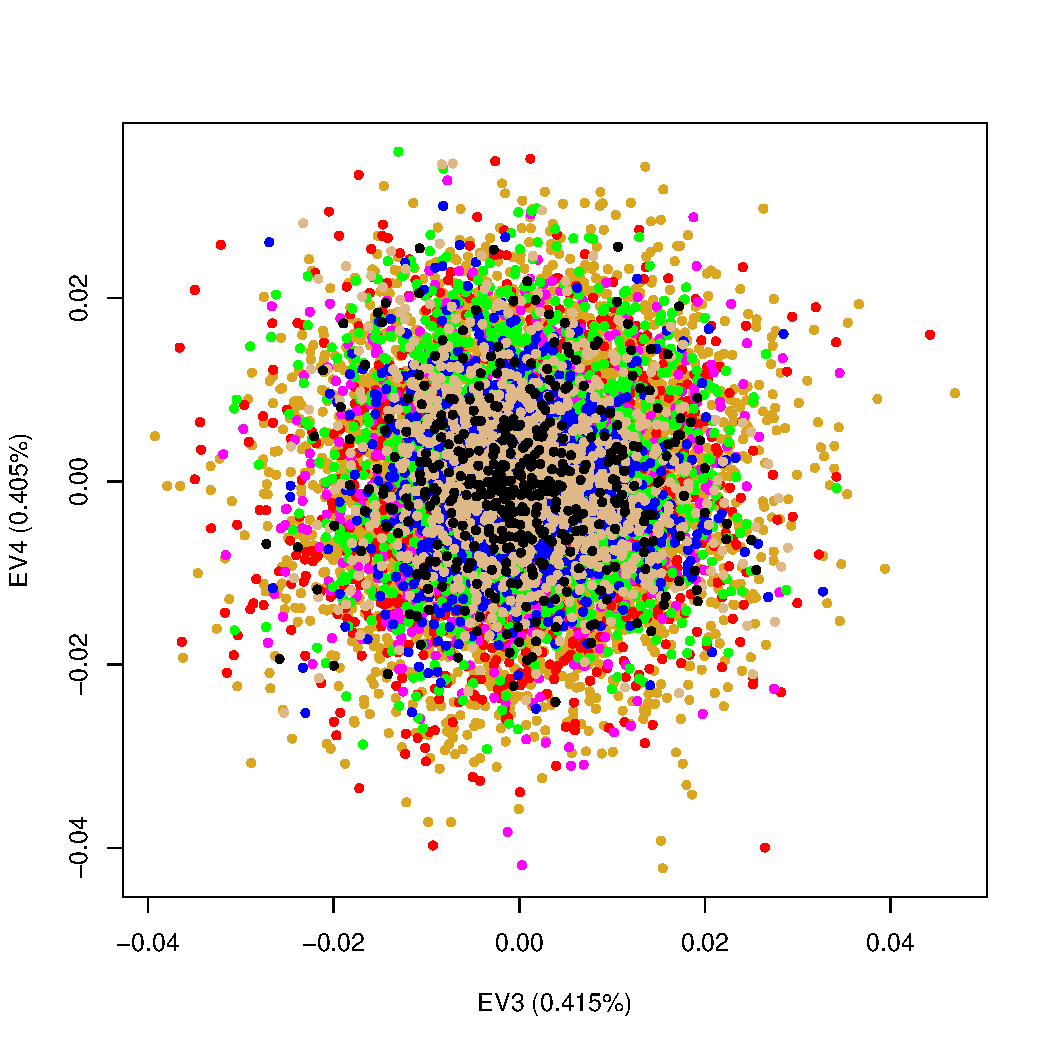
\includegraphics[height=8.5cm]{../pca_chr20_ev34_col.pdf}
\end{figure}
\end{frame}

\begin{frame}
\centering
\begin{figure}
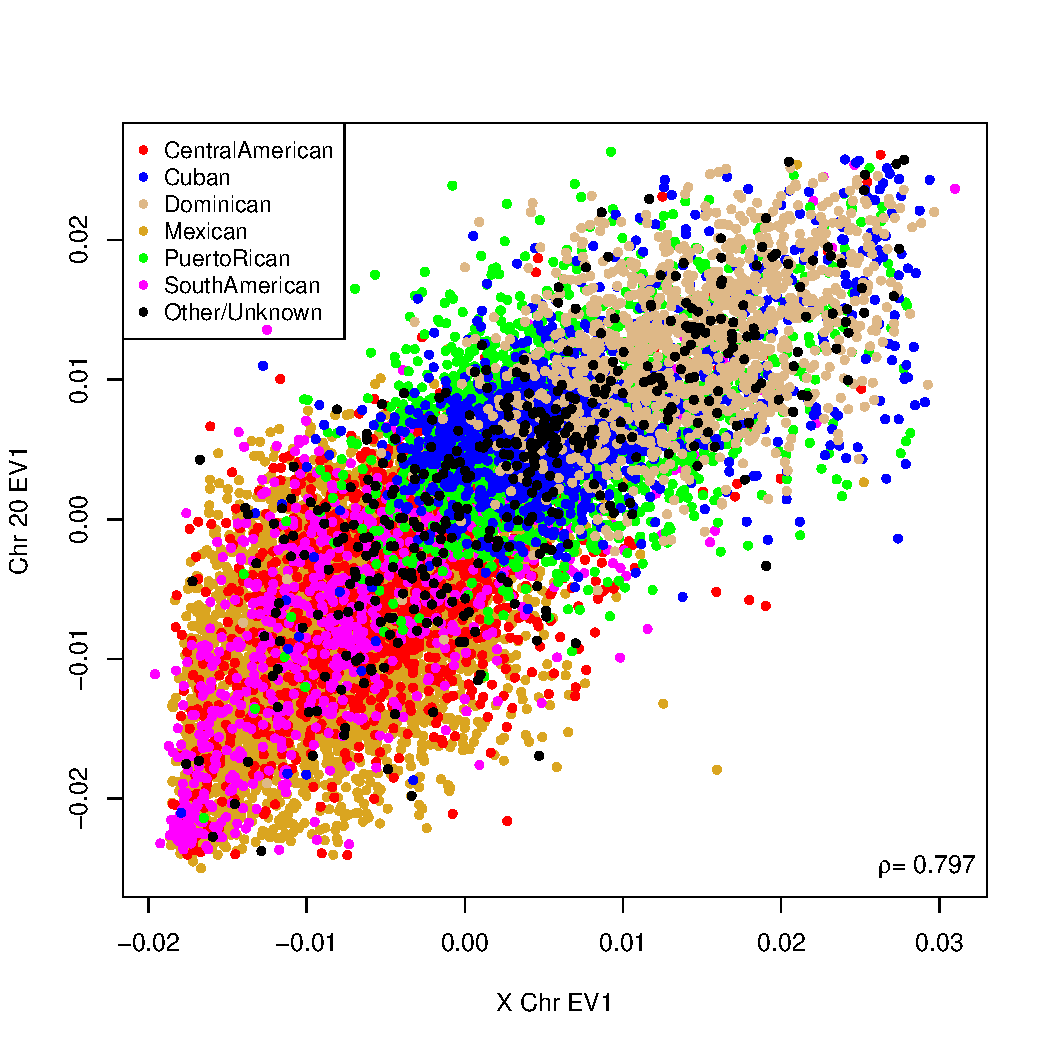
\includegraphics[height=8.5cm]{../pca_chr20_x_ev1_col.pdf}
\end{figure}
\end{frame}

\begin{frame}
\centering
\begin{figure}
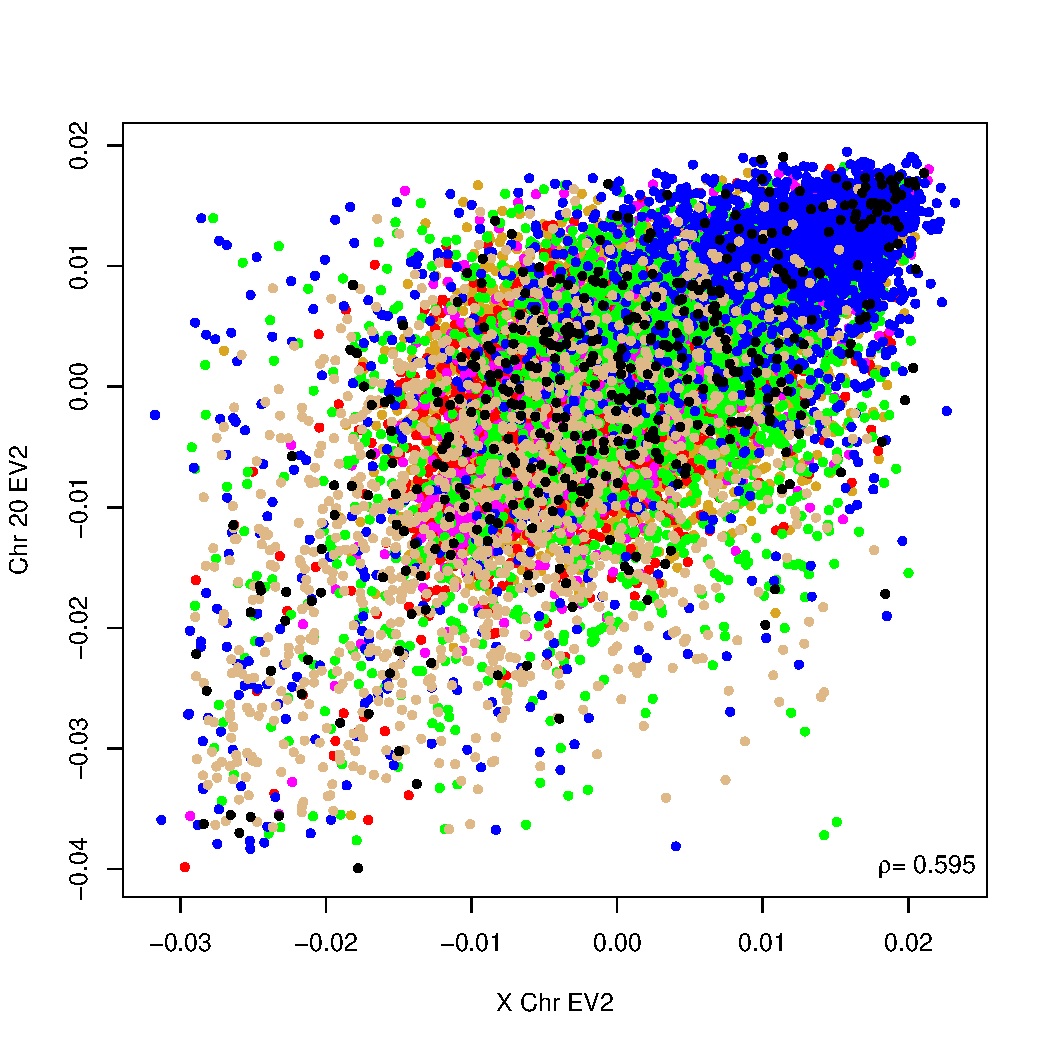
\includegraphics[height=8.5cm]{../pca_chr20_x_ev2_col.pdf}
\end{figure}
\end{frame}

\begin{frame}
\begin{itemize}
\item We examine results which use both 155,196 pruned autosomal and 3,582 pruned X chromosome SNPs together, for a total SNP set of 158,778 SNPs across the genome.
\end{itemize}
\end{frame}

\begin{frame}
\centering
\begin{figure}
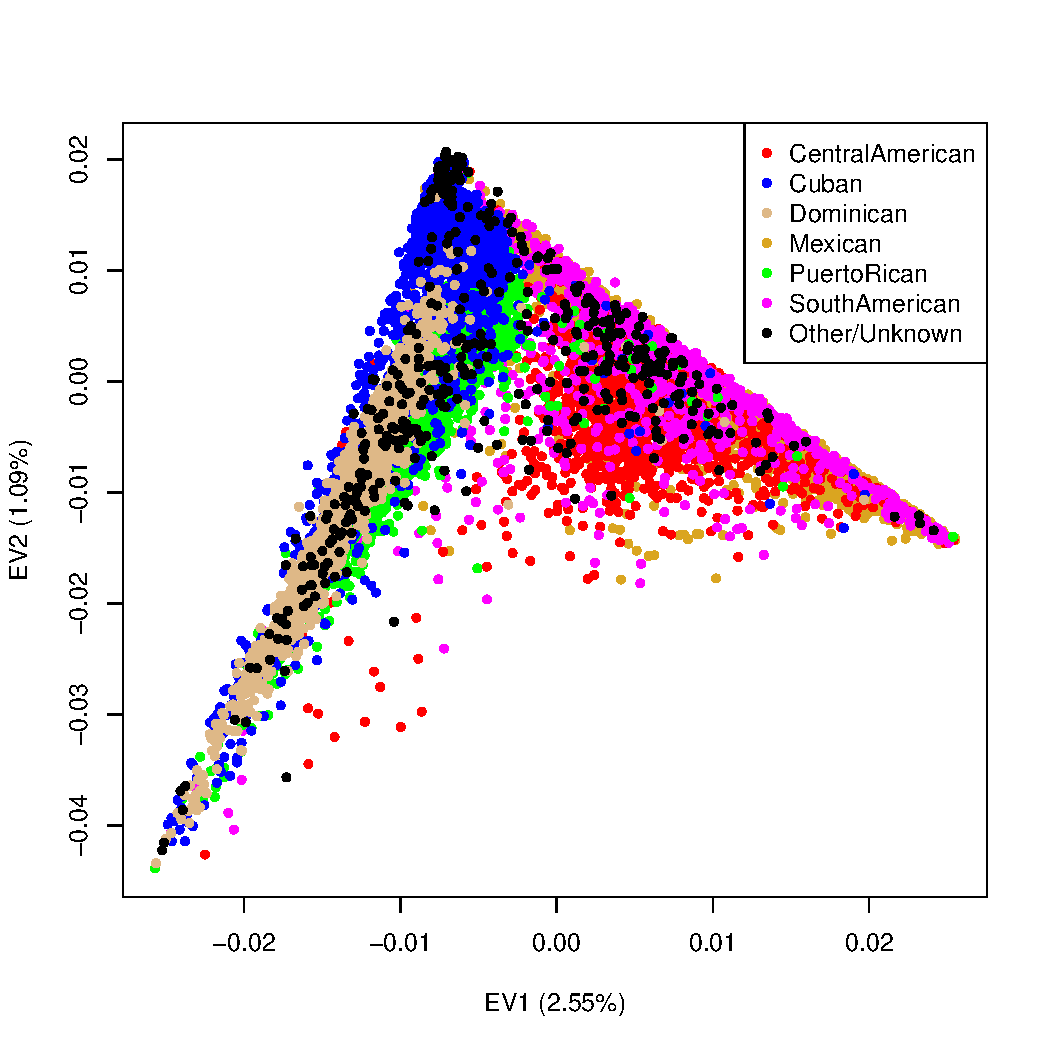
\includegraphics[height=8.5cm]{../pca_autoX_ev12_col.pdf}
\end{figure}
\end{frame}

\begin{frame}
\centering
\begin{figure}
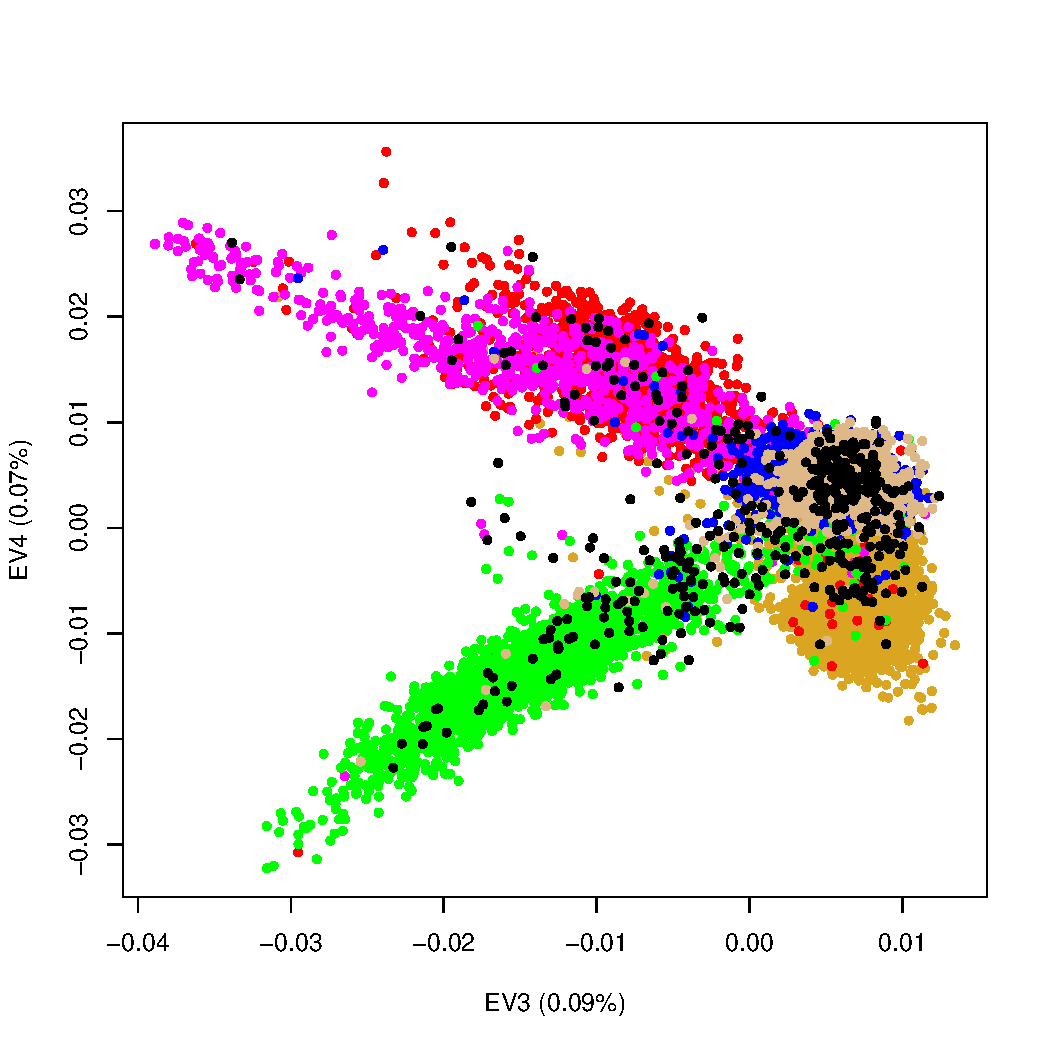
\includegraphics[height=8.5cm]{../pca_autoX_ev34_col.pdf}
\end{figure}
\end{frame}

\begin{frame}
\centering
\begin{figure}
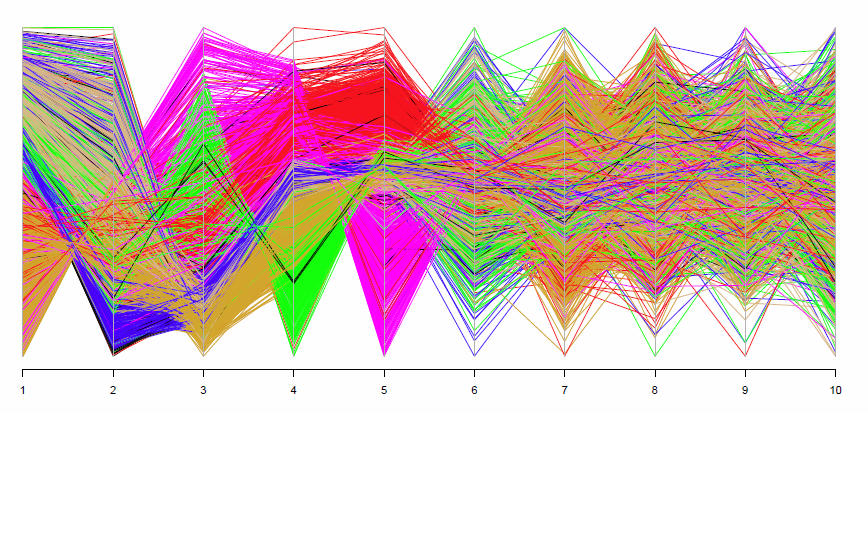
\includegraphics[height=7.5cm]{../pca_autoX_parCoords.png}
\end{figure}
\end{frame}

\begin{frame}
\centering
\begin{figure}
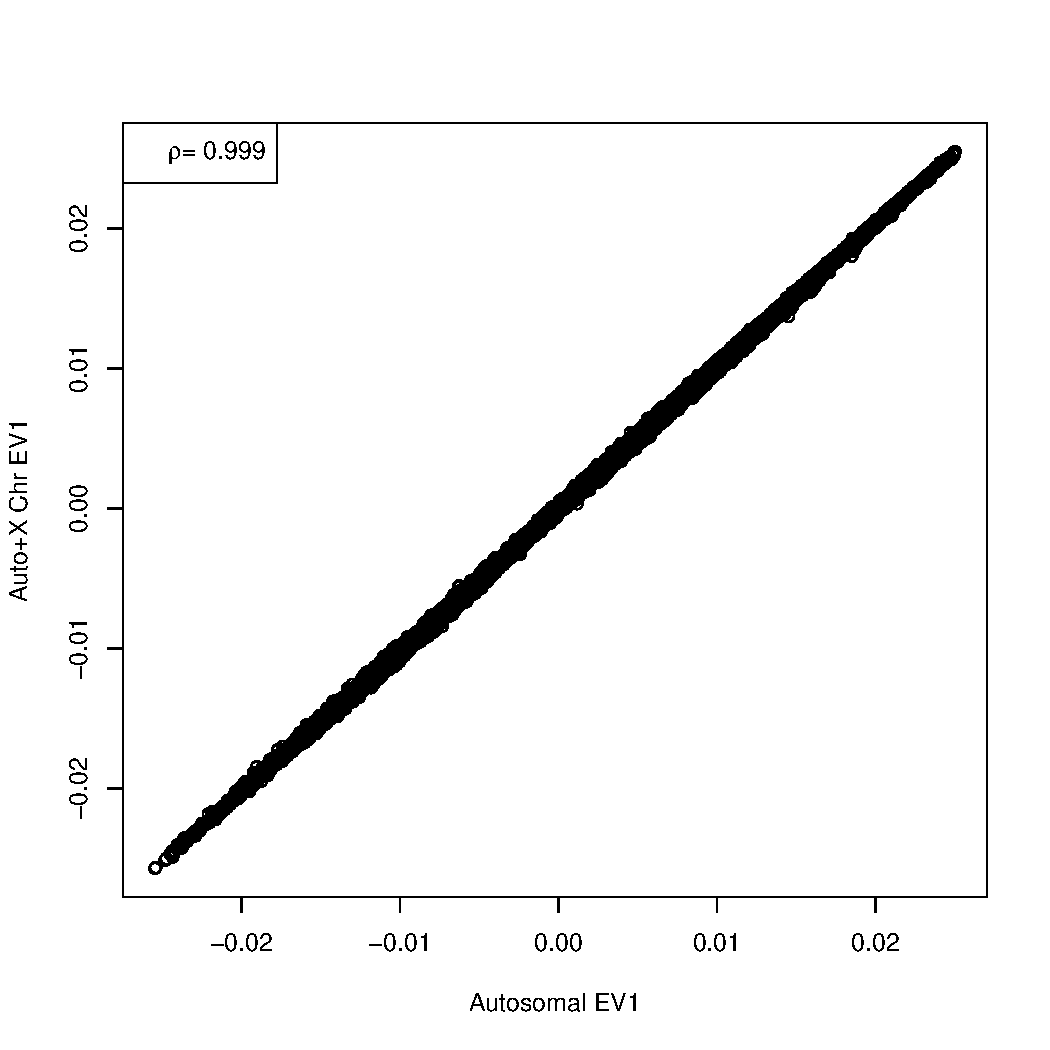
\includegraphics[height=8.5cm]{../pca_autoX_auto_ev1.pdf}
\end{figure}
\end{frame}



\begin{frame}
$\mathbf{\Phi_X}$ was estimated for all OLGA samples using the following scenarios:
\begin{table}[ht]
\centering
\begin{tabular}{r|ccc}
  \hline
   &SNP set& PCA run & EVs used \\ 
  \hline
1 &all X chr & - & - \\
2 & all X chr & autosomes + X chr & 1-5 \\
3 & all X chr & autosomes & 1-5\\
4 & all X chr & X chr & 1-2\\ \hline
5 & pruned X chr & - & - \\
6 & pruned X chr & autosomes + X chr & 1-5\\
7 & pruned X chr & autosomes & 1-5\\
8 & pruned X chr & X chr & 1-2 \\
   \hline
9 & pruned autosomal & autosomes & 1-5\\
\end{tabular}
\end{table}
All settings used the autosomal unrelated set of 10,272 samples and estimated $\mathbf{\Phi_X}$ for 12,734 study samples posted to dbGaP with no X chromosome anomalies.
\end{frame}

\begin{frame}
\footnotesize Estimate of $\mathbf{\Phi_X}$ in 10,272 autosomal-unrelated samples \\
models 1-4: unpruned X chr SNPs \hspace{1.5cm} models 5-8: pruned X chr SNPs
\centering
\begin{figure}
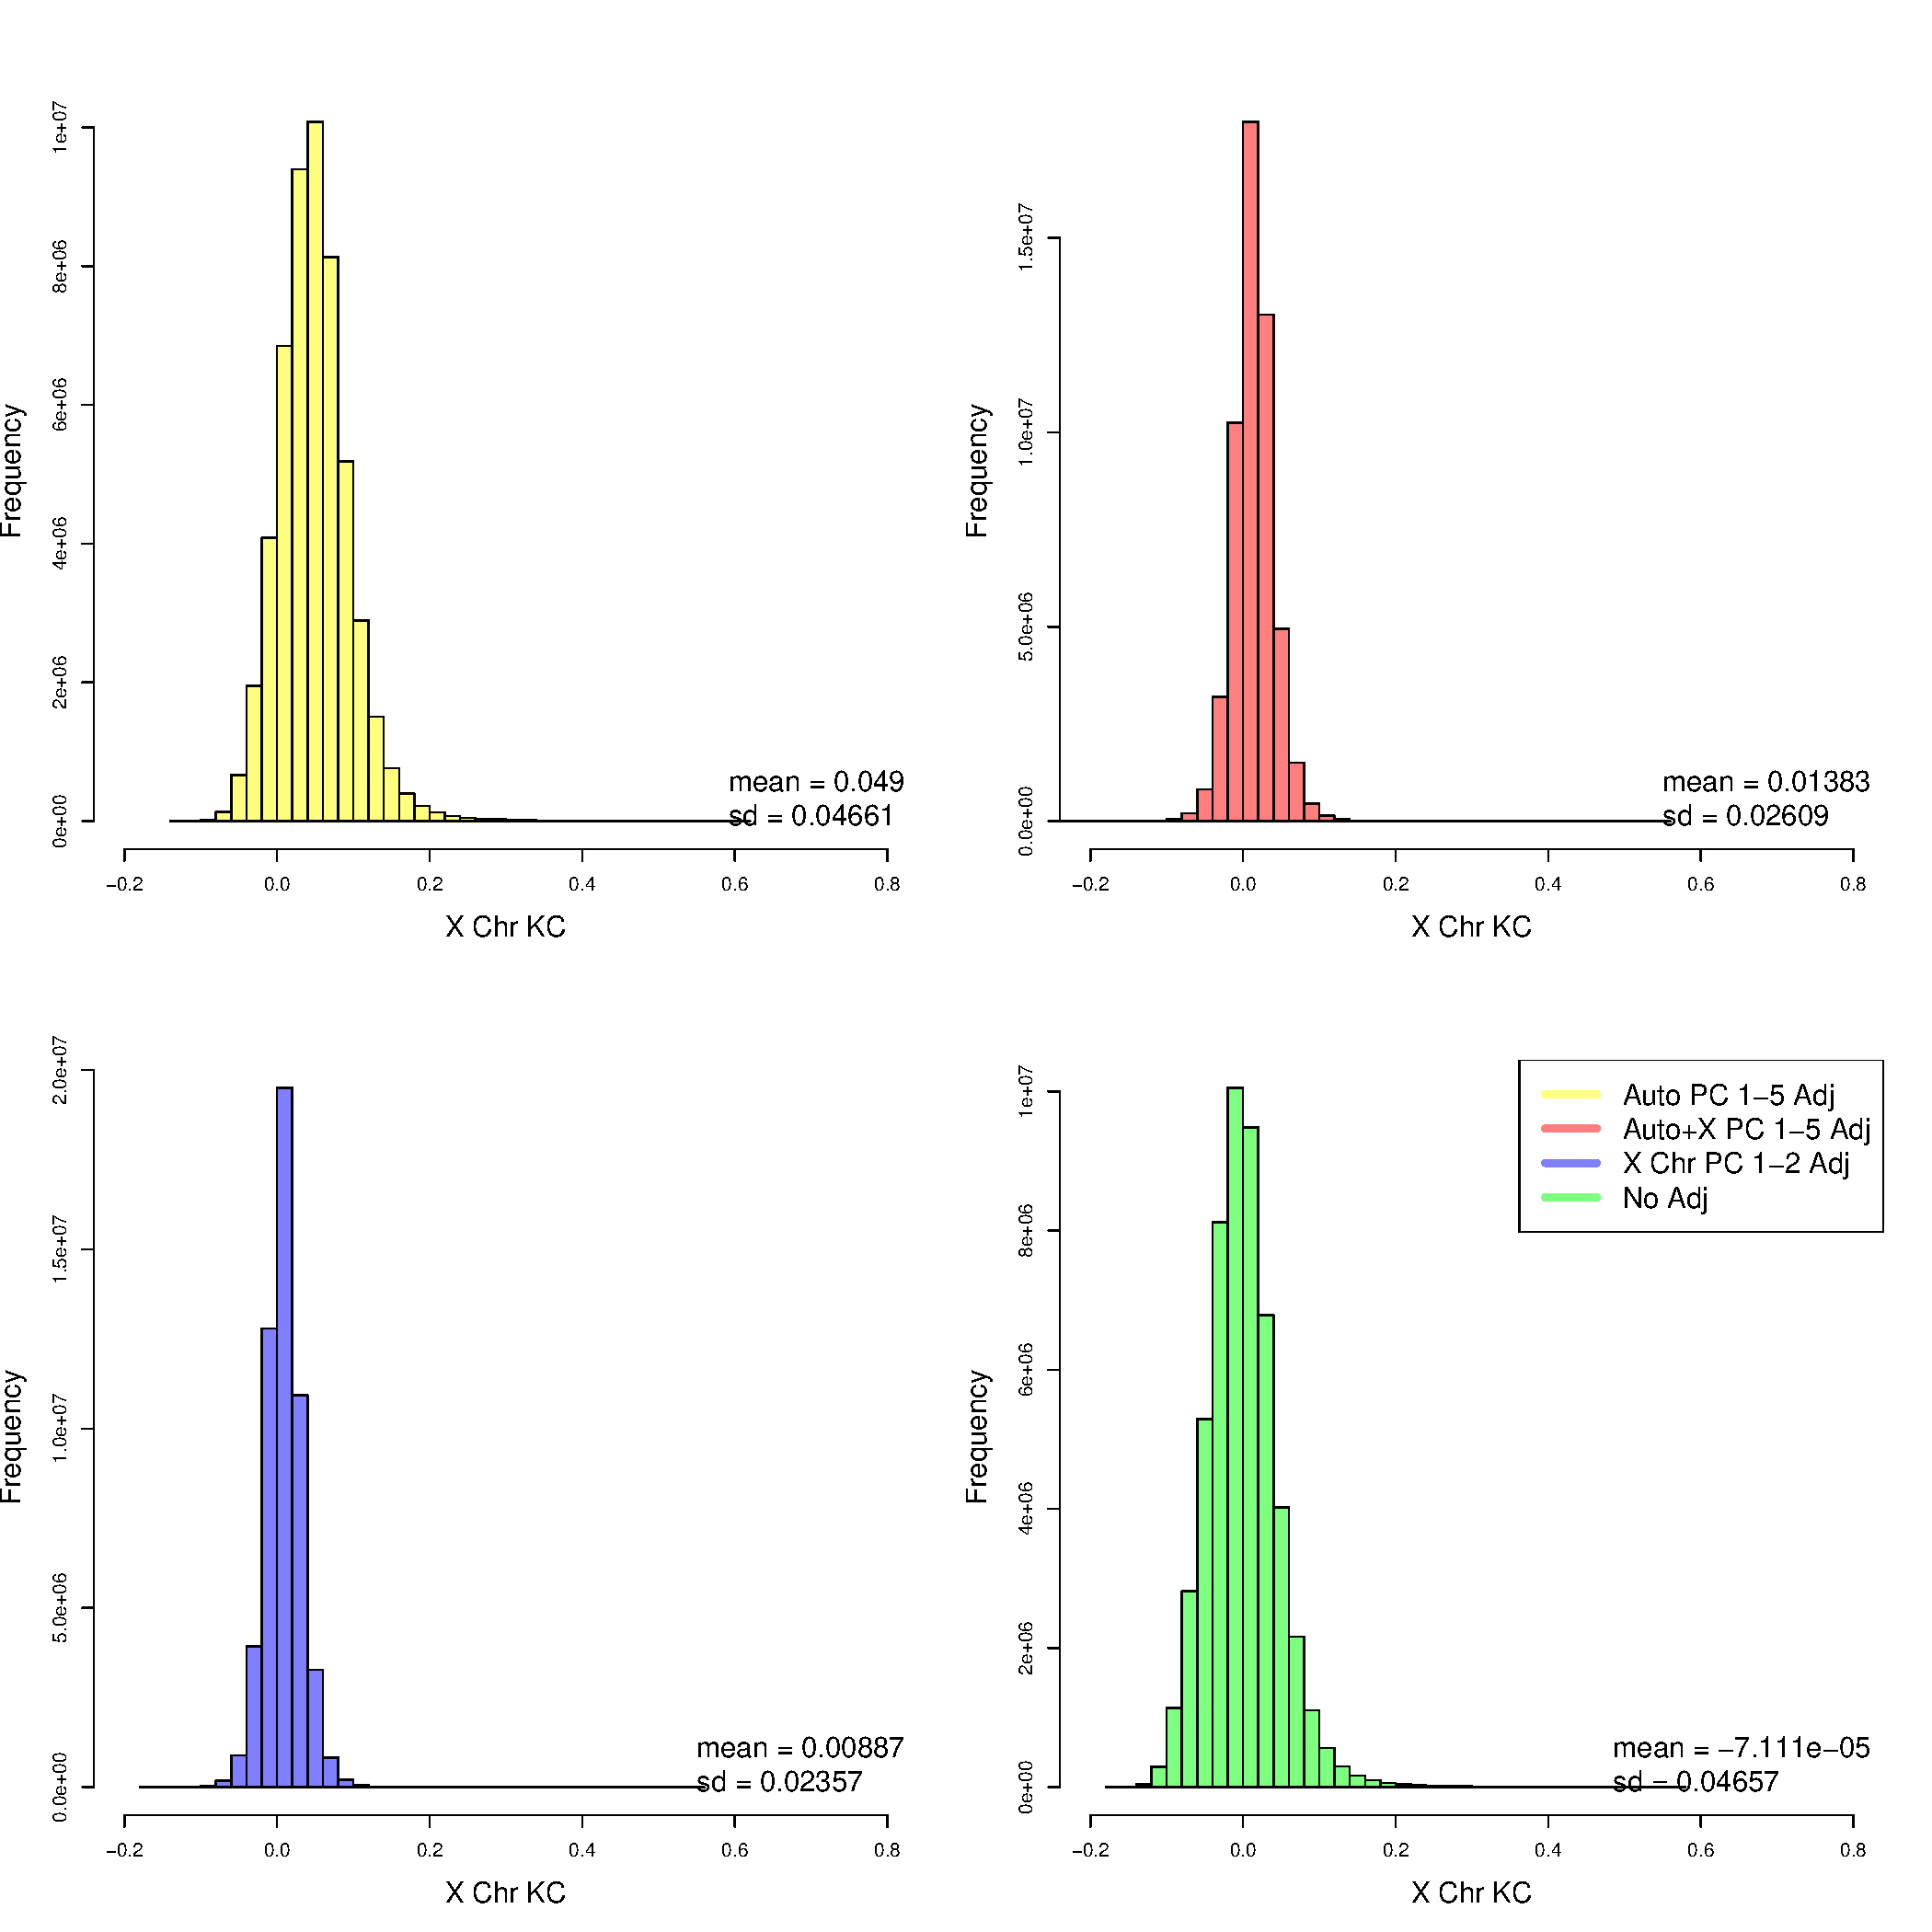
\includegraphics[height=6cm]{../hist_allXchrKC.pdf} \vline
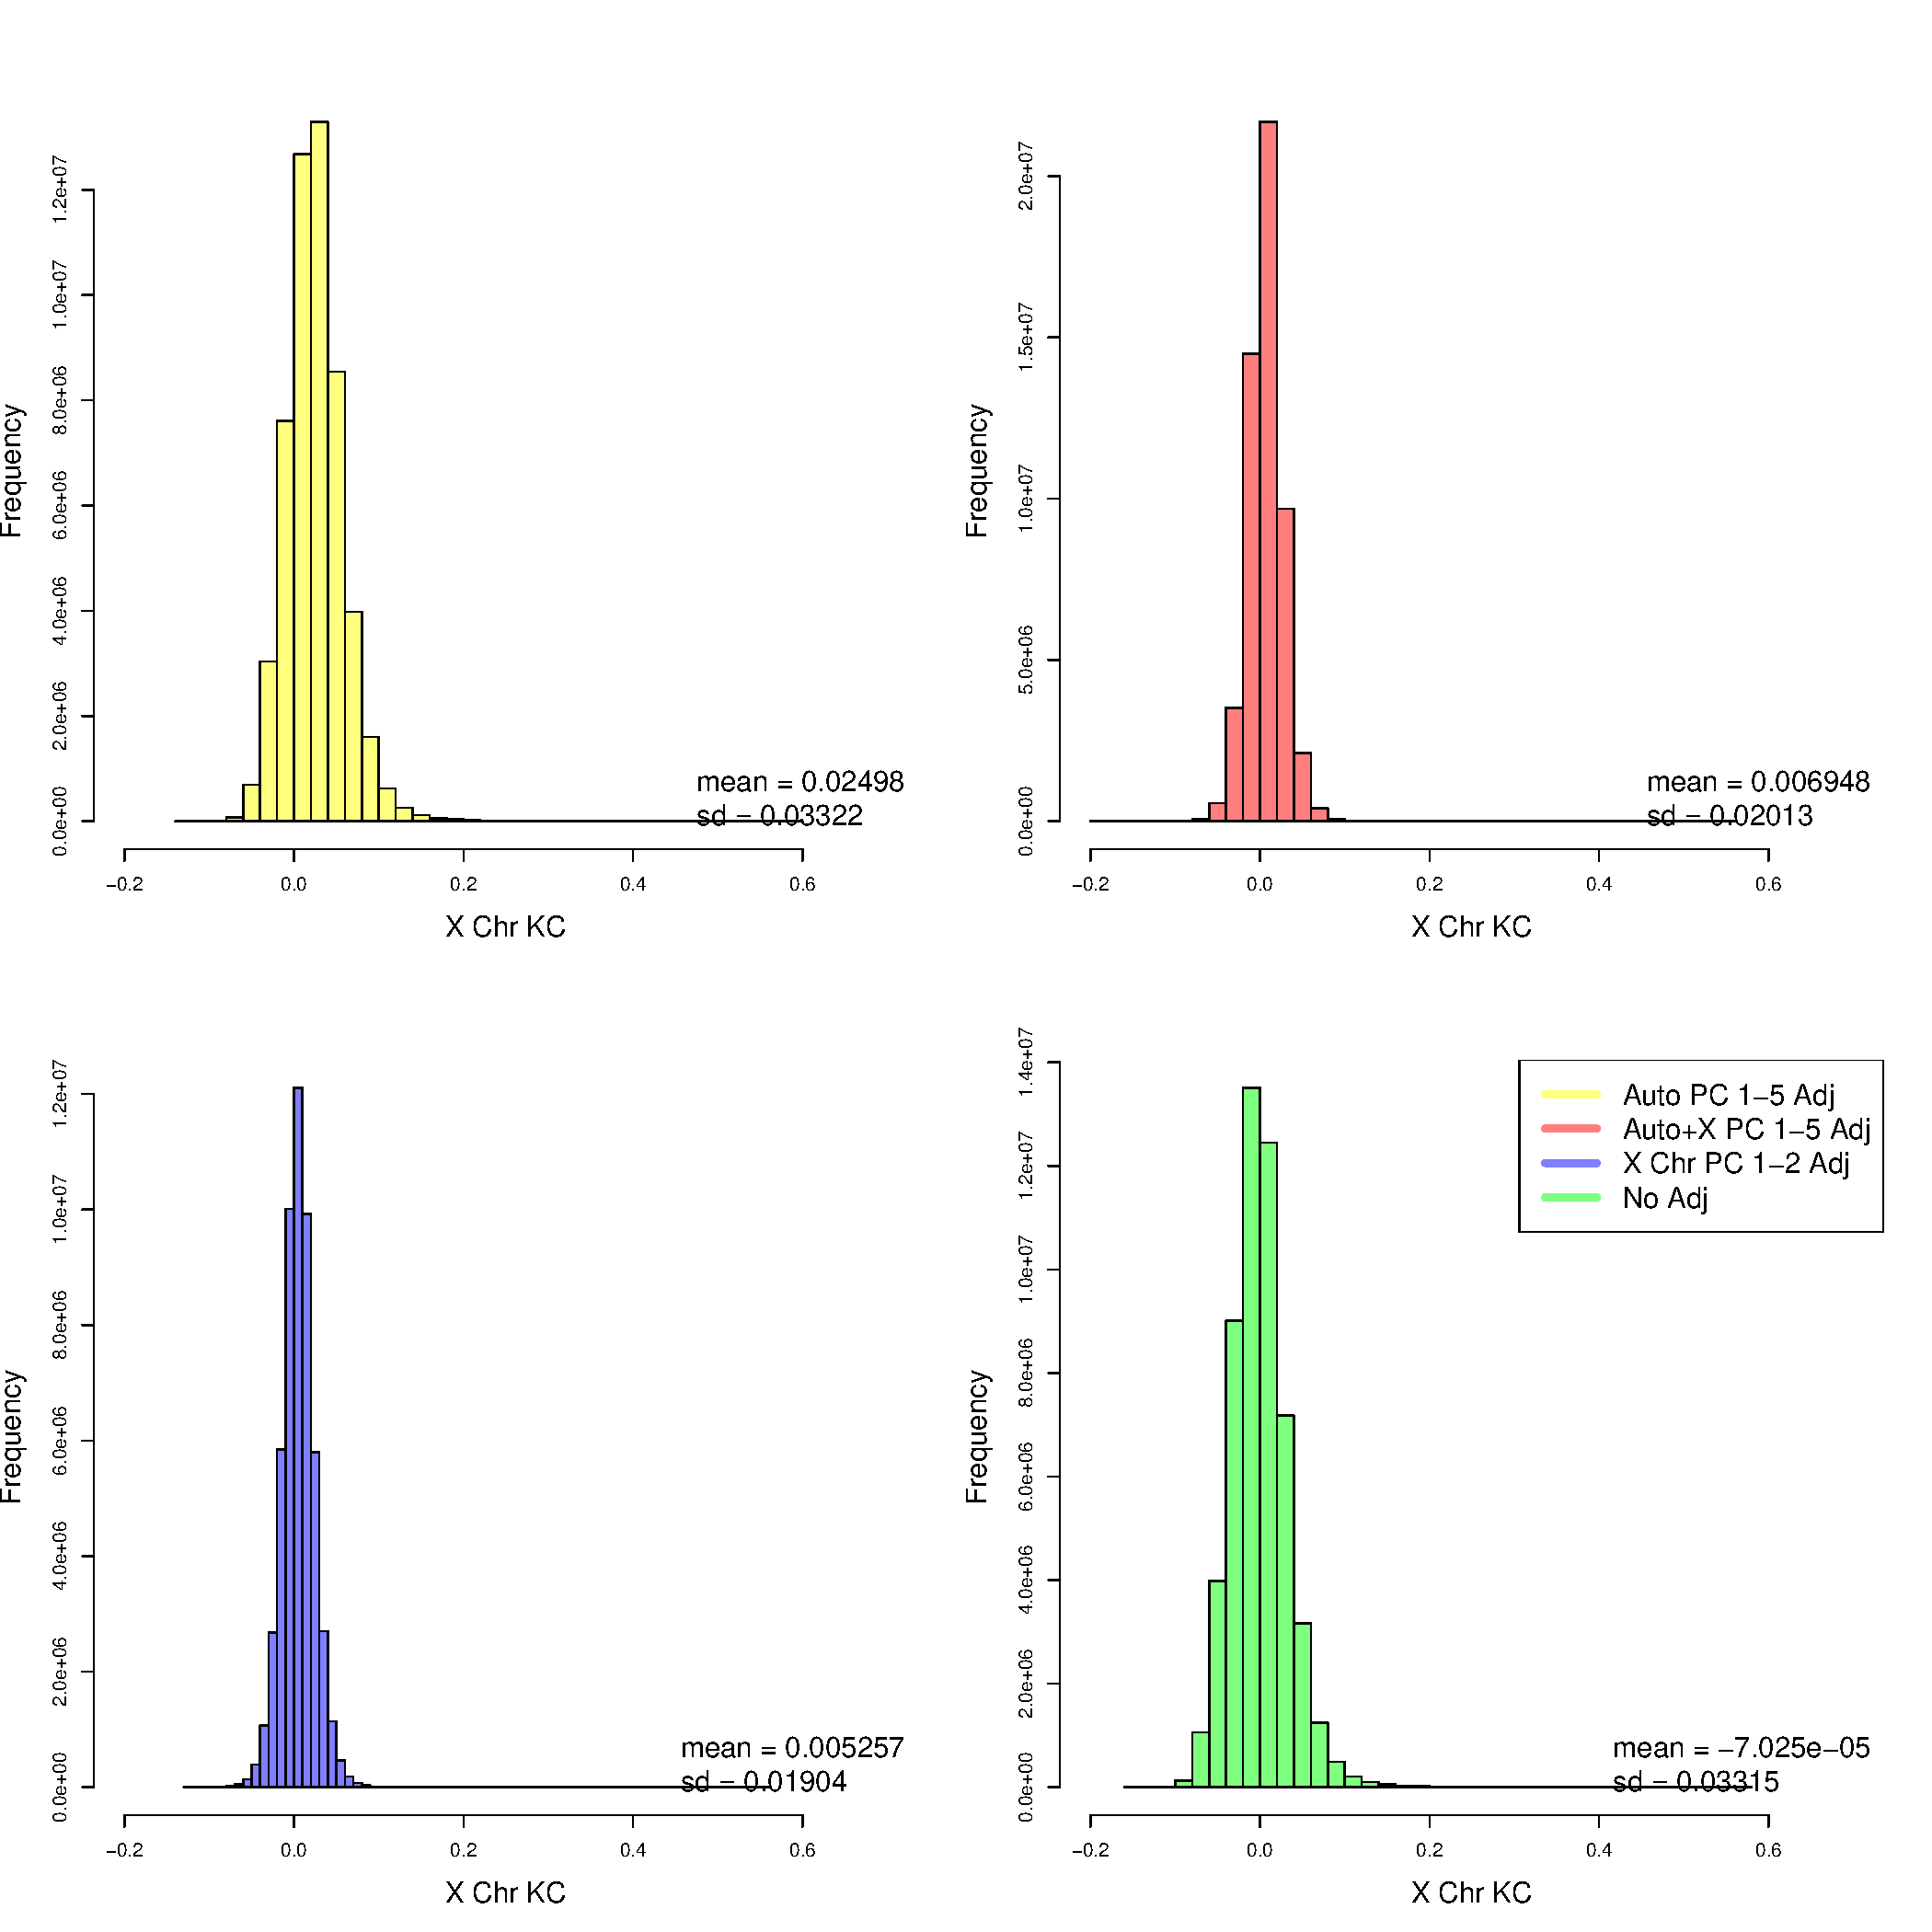
\includegraphics[height=6cm]{../hist_allXPrunedKC.pdf}
\end{figure}
\end{frame}

\begin{frame}
\footnotesize 
Unadjusted \hspace{5cm} Auto PC 1-5 Adjusted
\centering
\begin{figure}
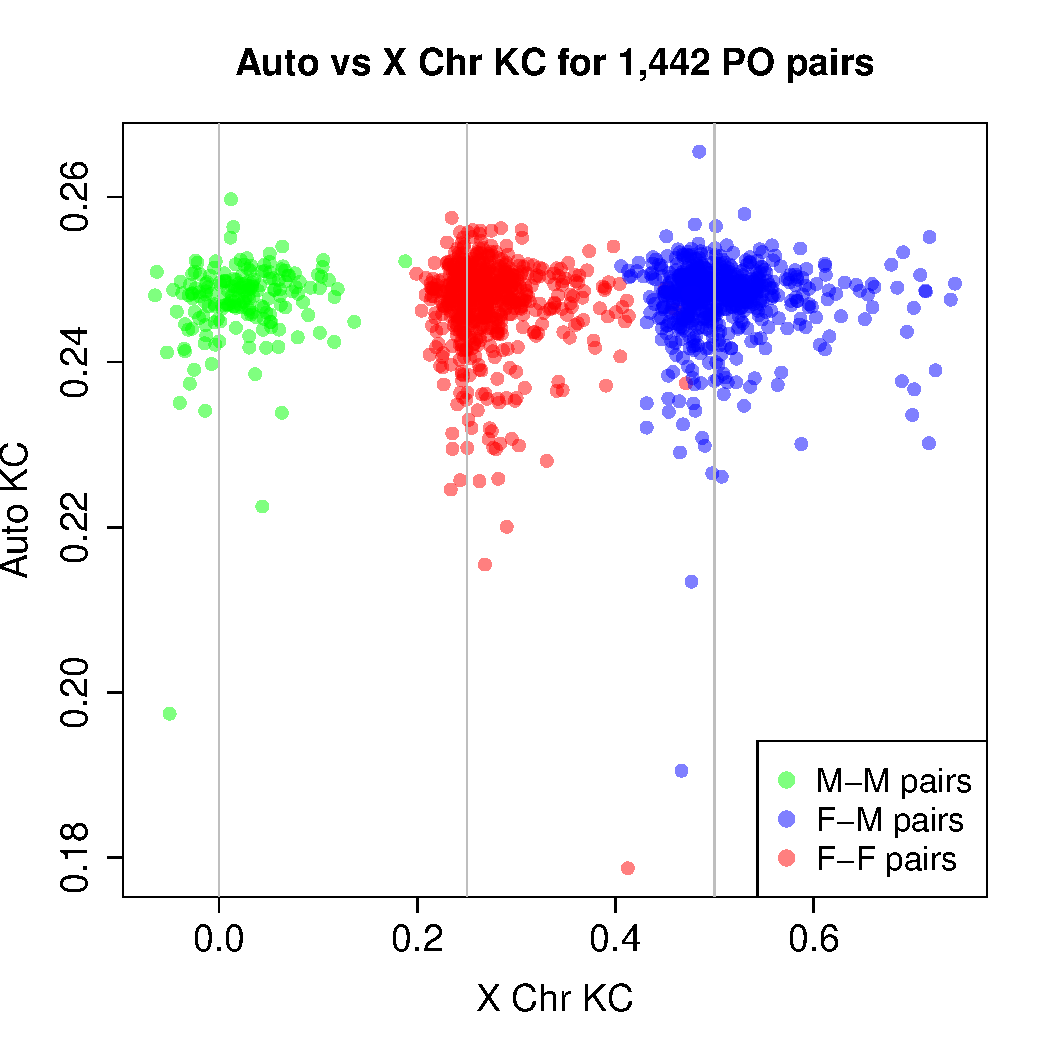
\includegraphics[height=6cm]{../kc_xPrunedvsAuto_poPairs_unadj.pdf}
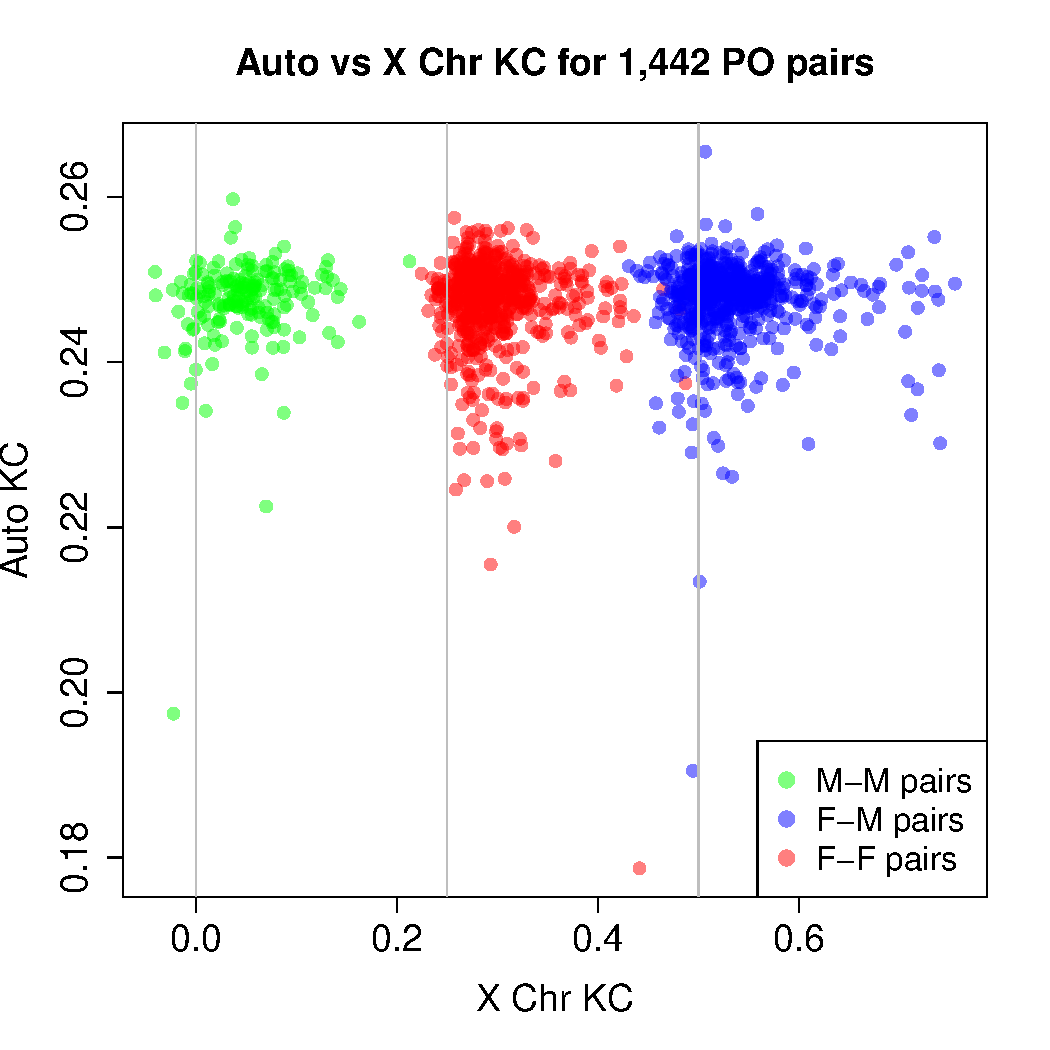
\includegraphics[height=6cm]{../kc_xPrunedvsAuto_poPairs_autoPC15adj.pdf}
\end{figure}
\end{frame}

\begin{frame}
\footnotesize
Auto + X PC 1-5 Adjusted \hspace{4cm} X PC 1-2 Adjusted
\centering
\begin{figure}
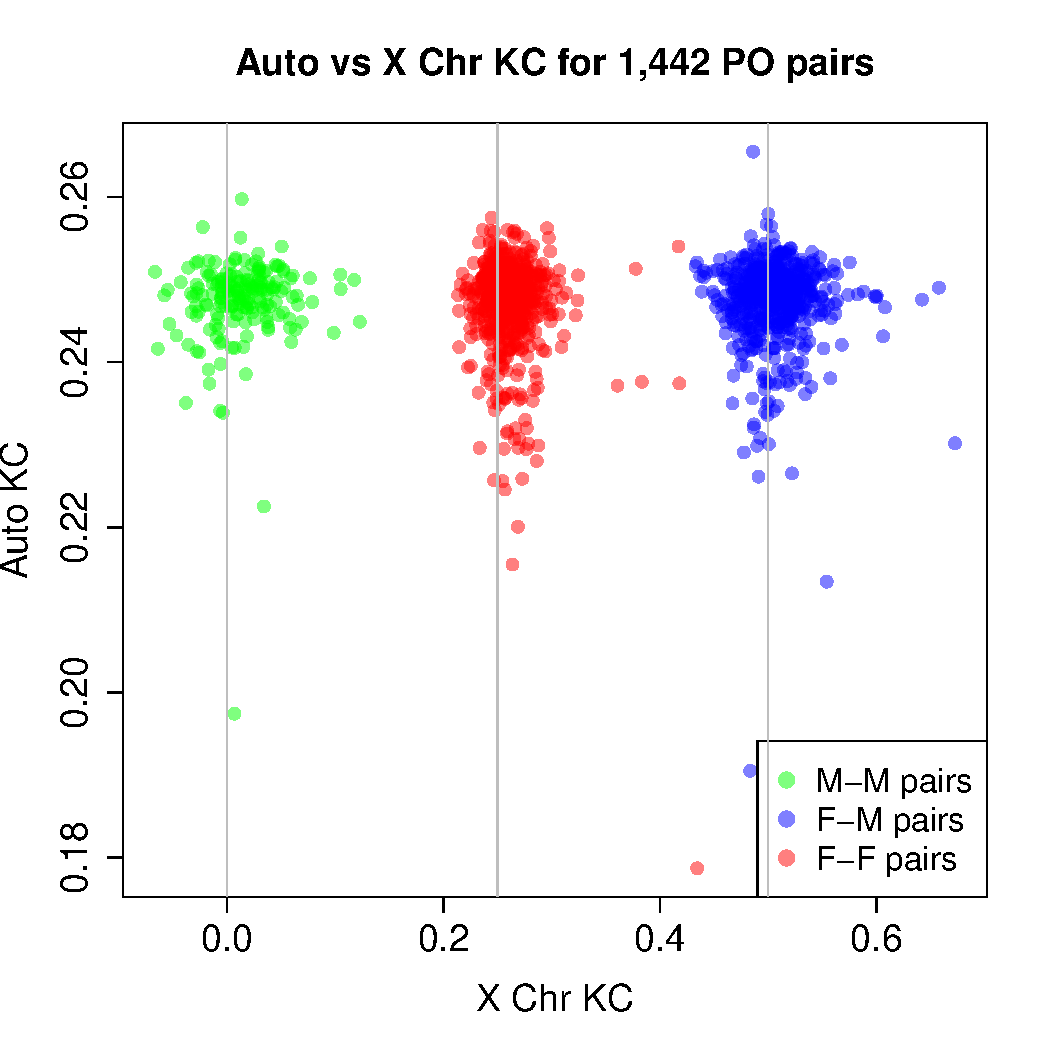
\includegraphics[height=6cm]{../kc_xPrunedvsAuto_poPairs_autoXAdj.pdf}
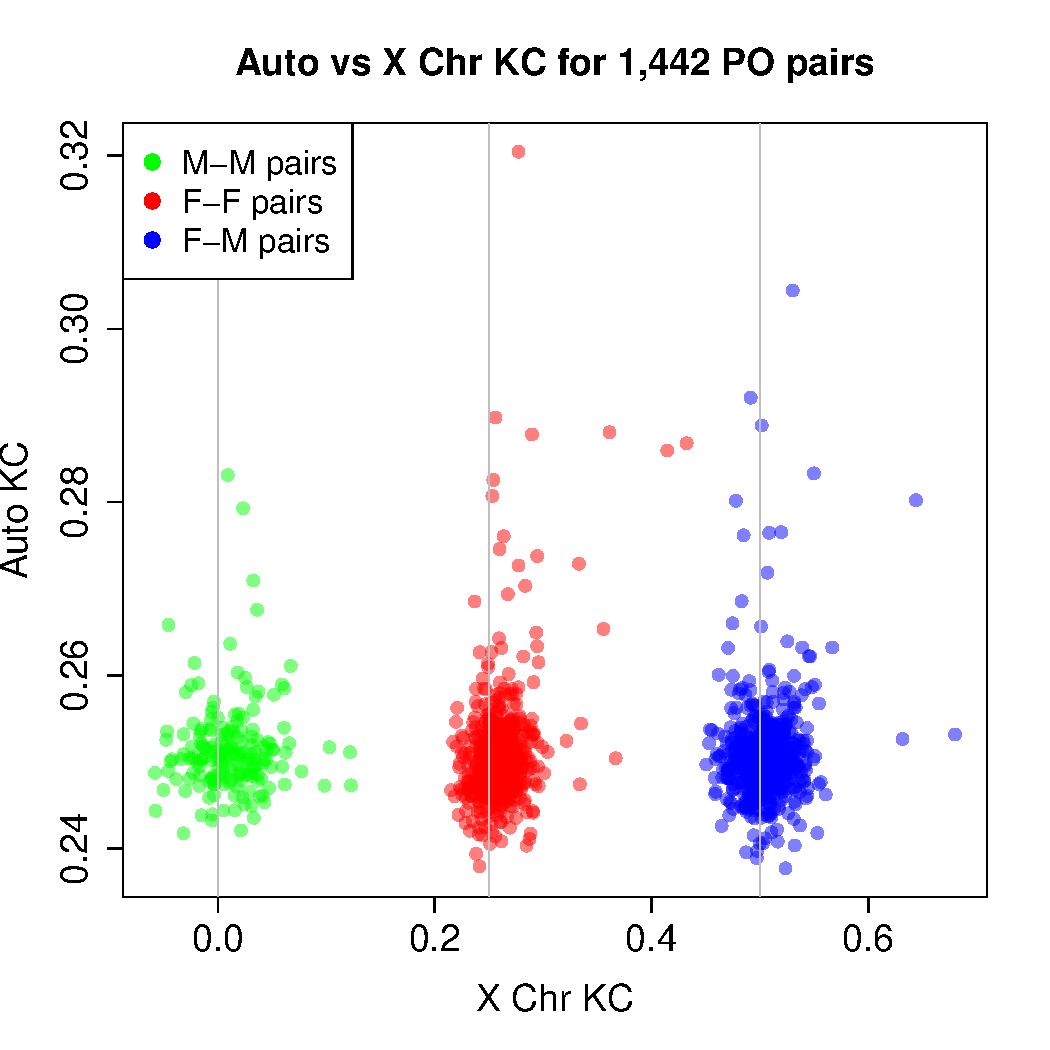
\includegraphics[height=6cm]{../kc_xPrunedvsAuto_poPairs_xAdj.pdf}
\end{figure}
\end{frame}

\begin{frame}
\begin{itemize}
\item We calculate PCs using a pruned set of autosomal SNPs.
\item We then estimate $\mathbf{\Phi_X}$ using a pruned set of X chromosome SNPs, adjusting for PCs 1-5 on the autosomes.
\item We then calculate PCs using a pruned set of X chromosome SNPs, adjusting for the calculated $\mathbf{\Phi_X}$, which is adjusted for autosomal structure.
\item We consider $\mathbf{\Phi_X}$ thresholds of 0.025 and 0.2 for unrelated pairs.
\end{itemize}
\end{frame}

\begin{frame}
\footnotesize
Unrel threshold 0.025 \hspace{4cm} Unrel threshold 0.2
\centering
\begin{figure}
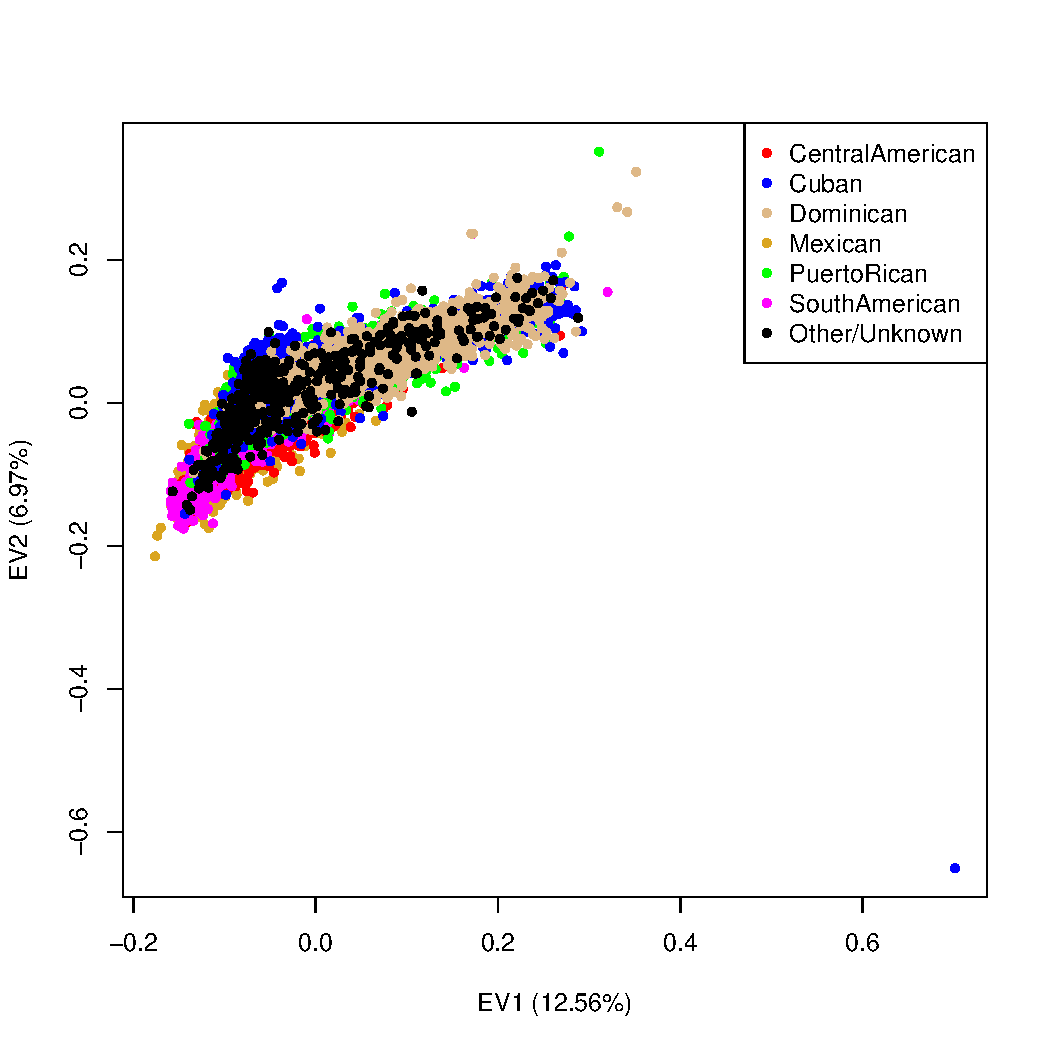
\includegraphics[height=6cm]{../pca_X_adjXkc_adjAutoXPC15_ev12_col.pdf}
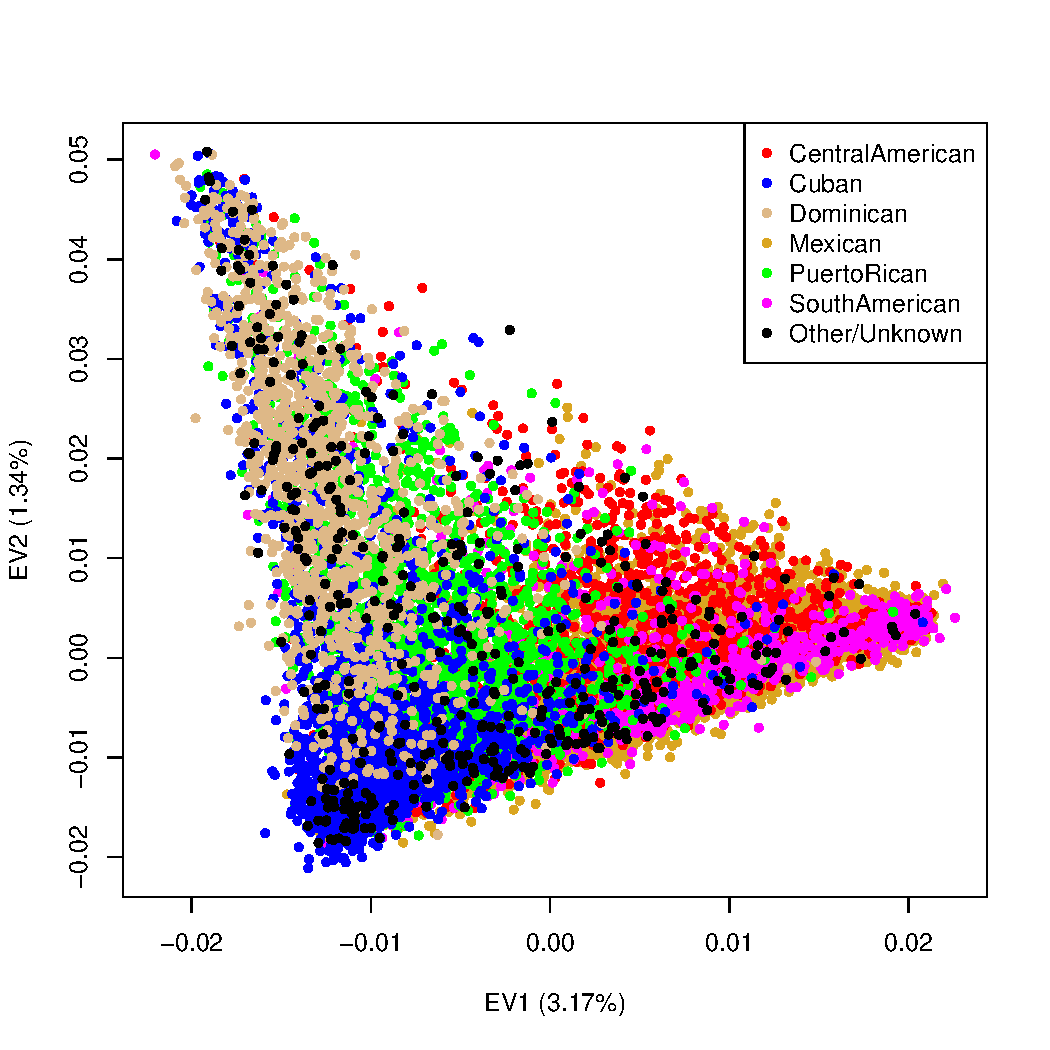
\includegraphics[height=6cm]{../pca_prunedX_adjXkc_adjAutoPC15_xPrunedKC_ev12_col.pdf}
\end{figure}
\end{frame}

\begin{frame}
\footnotesize
Unrel threshold 0.025 \hspace{4cm} Unrel threshold 0.2
\centering
\begin{figure}
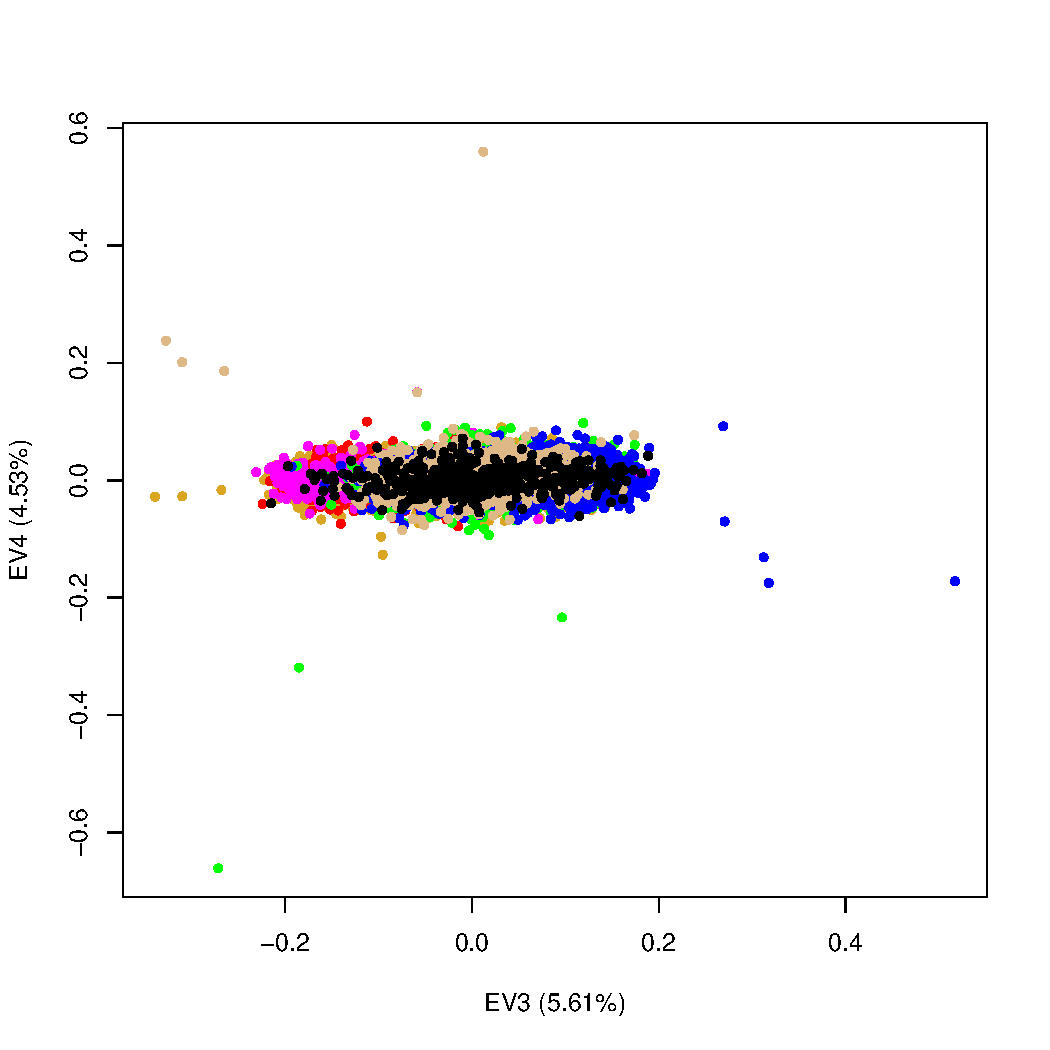
\includegraphics[height=6cm]{../pca_X_adjXkc_adjAutoXPC15_ev34_col.pdf}
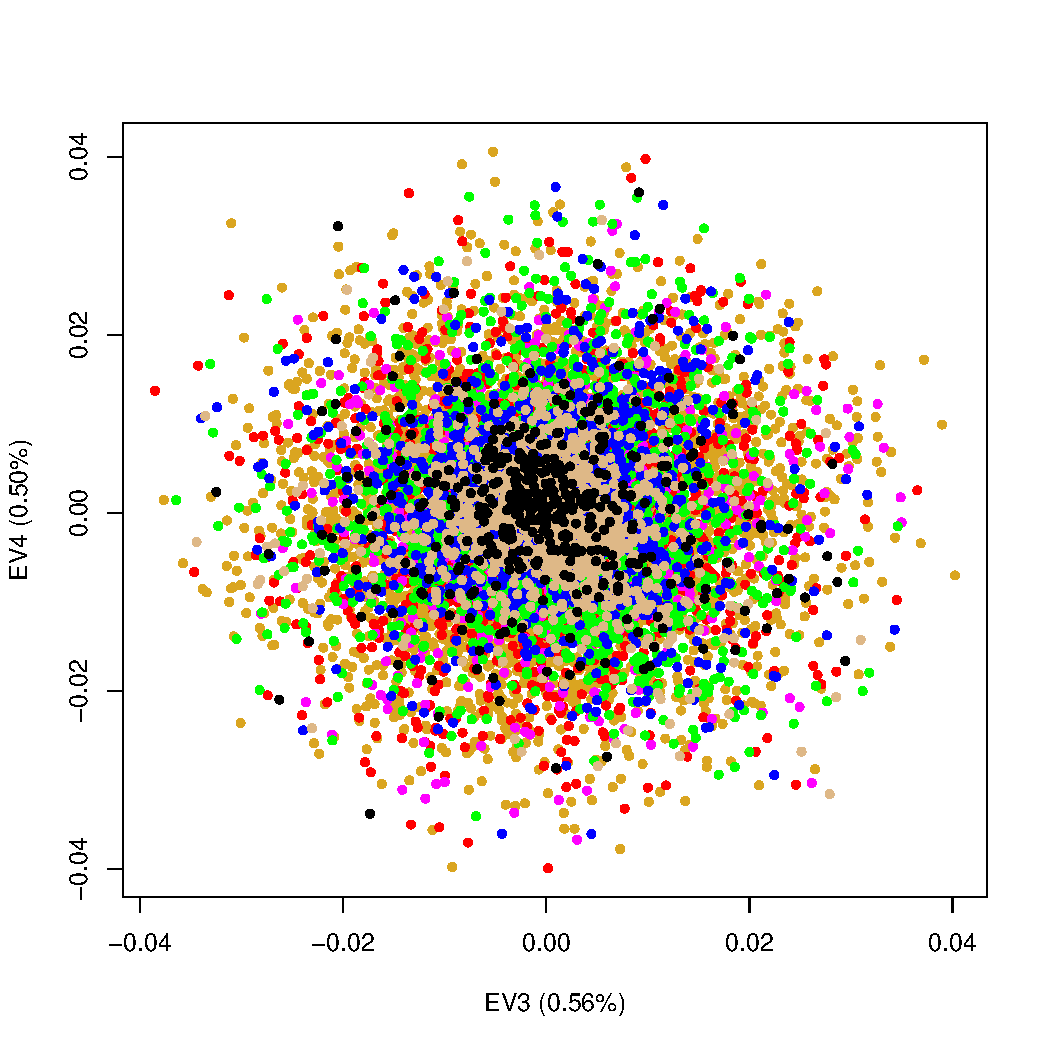
\includegraphics[height=6cm]{../pca_prunedX_adjXkc_adjAutoPC15_xPrunedKC_ev34_col.pdf}
\end{figure}
\end{frame}

\end{document}


